\newif\ifseminararbeit
\newif\ifblockingnotice
% Hier müssen die Variablen angepasst werden
% Der Titel der Arbeit, der auf dem Deckblatt angezeigt wird
\def \thesisTitle {Passwort Hacking: Vergleich von Brute-Force-Angriffen, Dictionary-Angriffen und Rainbow Tables zur Authentifizierungssicherheit}

% Der Titel der Arbeit, der in der Fußzeile angezeigt wird
\def \thesisFooterTitle {Passwort Hacking: Vergleich von Brute-Force-Angriffen, Dictionary-Angriffen und Rainbow Tables zur Authentifizierungssicherheit}

% Typ der Arbeit
\def \thesisType {Seminararbeit}

% Bildungsabschluss
\def \degree {Bachelor of Science}

% Abgabedatum
\def \submissionDate {6. Juni 2023}

% Studiengang
\def \courseOfStudies {Informatik}

% Kurs
\def \course {TIF21B}

% Name des Autors der Arbeit
\def \name {Marvin Obert}

% Name der Ausbildungsfirma
\def \company {VEGA Grieshaber KG}

% Ort, an dem Ausbildungsfirma ansässig ist
\def \companyLocation {Schiltach}

% Betreuer der Ausbildungsfirma
\def \corporateAdvisor {Leonie Musterfrau}

% Wissenschaftlicher Betreuer
\def \universityAdvisor {Prof. Dr. Hans Mustermann}

% Ort und Datum für die Ehrenwörtliche Erklärung
\def \declarationLocation {Lörrach}
\def \declarationDate {15. Februar 2000}

% Ort und Datum für die Freigabe der Arbeit
\def \releaseLocation {Freiburg im Breisgau}
\def \releaseDate {01. Februar 2000}

% Name der Bilddatei für das Firmenlogo. Die Datei muss im Ordner images sein.
% Erlaubt sind u.a. folgende Formate: PDF, PNG, JPEG
\def \fileNameLogo {company_logo.pdf}

% Je nach Länge des Titels kann die Schriftgröße angepasst werden
\def \titleFontSize {18}		% Schriftgröße des Titels auf dem Deckblatt
\def \footerFontSize {9}		% Schriftgröße in der Fußzeile

% Wenn es sich um eine Seminararbeit handelt,
% muss der folgende Befehl durch diesen ersetzt werden:
\seminararbeittrue
%\seminararbeitfalse

% Wenn die Arbeit keinen Sperrvermerk hat,
% muss der folgende Befehl durch diesen ersetzt werden:
\blockingnoticefalse
%\blockingnoticetrue

% Die Daten für den Sperrvermerk. Diese müssen natürlich nur geändert werden,
% wenn die Arbeit einen Sperrvermerk hat.
% Datum der Unterschrift des Autors auf dem Sperrvermerk
\def \blockingNoticeAuthorDate {02. Februar 2000}
% Datum der Unterschrift des Unternehmensvertreters auf dem Sperrvermerk
\def \blockingNoticeCompanyDate {03. Februar 2000}
% Adresse und Land des Unternehmens auf dem Sperrvermerk. Die \\ sorgen für einen Zeilenumbruch
\def \companyAdress {Talstraße 1 \\ 79539 Lörrach \\ Deutschland}
% Telefonnummer des Unternehmens auf dem Sperrvermerk.
\def \companyPhone {07621 20710}
% E-Mailadresse des Unternehmens auf dem Sperrvermerk.
\def \companyEmail {info@musterfrau-ag.de}
\documentclass[a4paper,12pt]{article}
\usepackage{fontspec}
\usepackage{polyglossia}
\usepackage{csquotes}
\setdefaultlanguage[spelling=new, babelshorthands=true]{german}

% Seitenränder
\usepackage[left=3.0cm, right=3.0cm, head=2.5cm, bottom=2.5cm, foot=1cm, includefoot]{geometry}

% Abkürzungsverzeichnis
\usepackage[printonlyused]{acronym}

% Gut formatierte Tabellen
\usepackage{tabulary}

% Positioniert Tabellen und Abbildungen
\usepackage{float}

% Fügt Abschnitte wie den Anhang oder die Kurzfassung dem Inhaltsverzeichnis hinzu
\usepackage{tocbibind}

% Ermöglicht Abbildungen in LaTeX
\usepackage{graphicx}
\graphicspath{ {images/} }

% Definiert die Farben für Tabellen im DHBW-Style
\usepackage[table]{xcolor}
\definecolor{tableHeading}{gray}{0.672}
\definecolor{tableOdd}{gray}{0.945}
\definecolor{tableEven}{gray}{0.859}
\arrayrulecolor{white}

% Schriftart Carlito. Sie ist fast identisch mit Calibri.
% Calibri ist auf Linux und MacOS nicht verfügbar. 
\usepackage{carlito}
\setmainfont{carlito}

% Fußzeile und Kopfzeile
\usepackage{fancyhdr}
\renewcommand{\headrulewidth}{0pt}
\renewcommand{\footrulewidth}{0.4pt}
\renewcommand{\footnotesize}{\fontsize{\footerFontSize}{\footerFontSize}\selectfont}
\fancyhead{}
\fancyfoot{}
\fancyfoot[R]{\hfill \fontsize{\footerFontSize}{\footerFontSize}\selectfont \thepage}
\fancyfoot[C]{
    \parbox{0.8\textwidth}{
    \setlength\topsep{0pt}
    \begin{center}
    \fontsize{\footerFontSize}{\footerFontSize}\selectfont \thesisFooterTitle
    \end{center}
    }
}


% Positioniert die Fußnoten fest am unteren Ende der Seite
\usepackage[bottom]{footmisc}

% Zeilenabstand: 1.5
\usepackage{setspace}
\setstretch{1.5}

% Literaturverzeichnis
\usepackage[natbib=true, backend=biber, style=authoryear, dashed=false]{biblatex}
\DeclareBibliographyAlias{interview}{misc}
\addbibresource{text/bibliography.bib}

% Das Paket hyperref muss als letztes Paket geladen werden. Das Paket setzt Links im PDF-Dokument.
\usepackage[hidelinks, unicode]{hyperref}
\hypersetup{pdftitle = {\thesisTitle}, pdfauthor = {\name}}

% Normale Schriftart für URLs
\renewcommand{\UrlFont}{}

% Variable für das Speichern der Seitenzahl (römisch -> arabisch -> römisch)
\newcounter{pageNumber}

% Nummerierung: 2.1, 2.2 usw.
\renewcommand{\labelenumii}{\theenumii}
\renewcommand{\theenumii}{\theenumi.\arabic{enumii}.}

% Bei Bedarf können die Überschriften geändert werden
\def \declarationHeading{Ehrenwörtliche Erklärung}
\def \thesisSizeHeading{Hinweis zum Umfang der Arbeit}
\def \releaseHeading{Freigabe der Arbeit}
\def \blockingHeading{Sperrvermerk}
\def \abstractHeading{Kurzfassung}
\def \appendixHeading{Anhang}
\def \referenceHeading{Quellenverzeichnis}
\def \acronymHeading{Abkürzungsverzeichnis}

% Befehl für ein einleitendes Zitat
\newcommand{\epigraph}[2]{
    \begin{quote}\begin{quote}
        \begin{center}
            \textit{#1}
        \end{center}
        \hfill #2
    \end{quote}\end{quote}
}

\begin{document}
\thispagestyle{empty}
\vspace*{-3cm}
\ifseminararbeit
\else
\includegraphics[width=4.5cm]{\fileNameLogo}
\fi
\hfill

\includegraphics[width=4.5cm]{DHBW_logo.pdf}

\begin{center}
\vspace{0.5cm}
\fontsize{\titleFontSize}{\titleFontSize}\selectfont \thesisTitle \\
\ifblockingnotice
\vspace{0.5cm}
\textcolor{red}{mit Sperrvermerk}\\
\vspace{0.5cm}
\else
\vspace{2cm}
\fi
\thesisType \\
\vspace{2cm}
\normalsize für die Prüfung zum \\
\degree \\
\vspace{2cm}
des Studiengangs \courseOfStudies \\
an der \\
Dualen Hochschule Baden-Württemberg Lörrach \\
\vspace{1cm}
\name \\
\vspace{1cm}
\submissionDate \\
\vfill
\begin{tabular}{l l}
Kurs \hspace{1cm} & \course \\ 
Ausbildungsfirma \hspace{1cm} & \company, \companyLocation \\
\ifseminararbeit
\else 
Betreuer der Ausbildungsfirma \hspace{1cm} & \corporateAdvisor \\ 
\fi
Wissenschaftlicher Betreuer \hspace{1cm} & \universityAdvisor \\ 
\end{tabular} 
\end{center}

\pagenumbering{Roman}
\pagestyle{fancy}
\newpage

\begin{center}
\section*{\declarationHeading}
\addcontentsline{toc}{section}{\declarationHeading}
\end{center}
\noindent Ich versichere hiermit, dass ich meine Bachelorarbeit (bzw. Projektarbeit oder\linebreak Seminararbeit) mit dem Thema:

\begin{center}
\thesisTitle
\end{center}

\noindent selbstständig verfasst und keine anderen als die angegebenen Quellen und Hilfsmittel benutzt habe. Ich versichere zudem, dass die eingereichte elektronische Fassung mit der gedruckten Fassung übereinstimmt.

\vspace*{1.8cm}
\noindent \declarationLocation , \declarationDate \\
\vspace*{0.7cm} \\
\noindent\rule{8cm}{0.5pt} \\
\name \\
\vspace*{3cm} \\

\begin{center}
\section*{\thesisSizeHeading}
\addcontentsline{toc}{section}{\thesisSizeHeading}
\end{center}
Der Textteil der vorliegenden Arbeit - beginnend mit der Einleitung bis ausschließlich Quellenverzeichnis - umfasst \pageref{pagesForDeclaration} Seiten.
\newpage

\ifseminararbeit
\else
\begin{center}
\section*{\releaseHeading}
\addcontentsline{toc}{section}{\releaseHeading}
\end{center}
Die vorliegende Arbeit wurde durch das Ausbildungsunternehmen 
\company, {\companyLocation} inhaltlich geprüft und zur Vorlage an der DHBW Lörrach, Studiengang \courseOfStudies, freigegeben.

\vspace*{4cm}
\begin{center}
\begin{tabular}{c c}
\noindent\rule{7cm}{0.5pt} & \noindent\rule{7cm}{0.5pt} \\ 
\noindent \releaseLocation, \releaseDate & Unterschrift Unternehmensvertreter \\
\end{tabular} 
\end{center}
\newpage
\fi

\ifblockingnotice
\begin{center}
\section*{\textcolor{red}{\blockingHeading}}
\addcontentsline{toc}{section}{\blockingHeading}
\end{center}
Der Inhalt dieser Arbeit darf weder als Ganzes noch in Auszügen Personen außerhalb des Prüfungsprozesses und des Evaluationsverfahrens zugänglich gemacht werden, sofern keine anders lautende Genehmigung der Ausbildungsstätte vorliegt.
\vspace*{2cm}
\begin{center}
\begin{tabular}{c c}
\noindent\rule{7cm}{0.5pt} & \noindent\rule{7cm}{0.5pt} \\ 
\noindent \blockingNoticeAuthorDate, \name & \blockingNoticeCompanyDate, \company \\
\end{tabular} 
\end{center}
\vspace*{2cm}
Kontakt: \\
\company \\
\companyAdress \\
Tel.: \companyPhone \\
E-Mail: \companyEmail \\

\newpage
\fi

\section*{\abstractHeading}
\addcontentsline{toc}{section}{\abstractHeading}
Hier beginnt die Kurzfassung ihrer wissenschaftlichen Arbeit…
\newpage

\tableofcontents
\newpage

\section*{\acronymHeading}
\addcontentsline{toc}{section}{\acronymHeading}
\begin{acronym}

\acro{WPA2}{Wi-Fi Protected Access 2}
\acro{GPU}{Graphic Processing Unit}

\end{acronym}
\newpage

\listoffigures
\newpage

\listoftables
\newpage

\clearpage
\setcounter{pageNumber}{\value{page}}
\pagenumbering{arabic}

\rowcolors{1}{tableOdd}{tableEven}

% -----------------------------------------------------
% Hier sind die Kapitel.
% Bei Bedarf kann man Kapitel entfernen oder hinzufügen
\section{Einleitung}
\subsection{Einführung}
\epigraph{"`More companies are moving to new stronger technologies to authenticate user identities, like biometrics. Because it's just too easy for hackers to figure out usernames and passwords, like ``password``'' or 12345... 7. Those are some of my previous passwords. I've changed them since then."'}{Barack Obama\footcite[Vgl.]{CNET}}
In der heutigen Zeit sind Passwörter eine der grundlegendsten Methoden um Benutzer zu identifizieren. 
Allerdings ist die Komplexität der meisten Passwörter sehr gering und somit ist das Benutzernamen und Passwort erraten sehr leicht. 
Wie der ehemalige US-Präsident Barack Obama betont, haben Unternehmen erkannt, dass sie auf neue, stärkere Technologien umsteigen müssen, 
um die Identität von Benutzern zu authentifizieren, wie zum Beispiel biometrische Verfahren. 
Diese Authentifikationsmethoden sind angesicht der Passwörter des ehemalige Präsidenten ein deutlich stärkere und sichere Maßnahme.

\subsection{Zieldefinition}
Das Ziel dieser Seminararbeit besteht darin, eine umfassende Vergleichsanalyse ausgewählter Passwort-Hacking-Methoden durchzuführen. Dazu werden Brute-Force-Angriffe, Dictionary-Angriffe und Rainbow Tables im Hinblick auf Effizienz, Erfolgsrate und Ressourcenanforderungen untersucht. Zusätzlich erfolgt eine eingehende Untersuchung der Sicherheit des weit verbreiteten WLAN-Verschlüsselungsstandards WPA2 und der Diskussion möglicher Schutzmaßnahmen.

Um dieses Ziel zu erreichen, wird sowohl ein theoretischer Vergleich durchgeführt, bei dem eine Nutzwertanalyse erstellt wird, als auch ein praktischer Vergleich in einem konstruierten Testfall durchgeführt. Der praktische Vergleich ermöglicht eine Überprüfung der Wirksamkeit und Anwendbarkeit der verschiedenen Methoden.

Durch diese umfassende Herangehensweise soll ein fundiertes Verständnis für die Stärken und Schwächen der einzelnen Passwort-Hacking-Methoden gewonnen werden, 
um Empfehlungen für den Schutz vor solchen Angriffen abzuleiten. Die Kombination aus theoretischer Analyse und praktischer Anwendung ermöglicht eine ganzheitliche Betrachtung des Themas.
\subsection{Methodik}
\begin{enumerate}
  \item Einführung der gängigen Hacking-Methoden: Als erster Schritt erfolgt eine umfassende Einführung in die verschiedenen gängigen Hacking-Methoden. Dabei werden die Methoden ausführlich erläutert, um den Leserinnen und Lesern einen fundierten Überblick über die unterschiedlichen Angriffstechniken zu geben.
  \item Erklärung der Rainbow Tables: Im Anschluss daran erfolgt eine detaillierte Erklärung der Rainbow Tables, da diese für den praktischen Teil unverzichtbar sind. Es wird eine klare Definition der Rainbow Tables gegeben sowie ihre Funktionsweise und ihr Zweck im Kontext des Passwort-Hackings erläutert.
  \item Aufstellung von Vergleichskriterien: Nach der Einführung und Erläuterung der Hacking-Methoden werden spezifische Vergleichskriterien aufgestellt, anhand derer die verschiedenen Methoden verglichen werden können. Dadurch wird eine strukturierte Grundlage für den Vergleich geschaffen.
  \item Durchführung einer Nutzwertanalyse: Im nächsten Schritt erfolgt die Durchführung einer Nutzwertanalyse, um die verschiedenen Hacking-Methoden anhand der aufgestellten Kriterien zu bewerten. Dadurch können die Vor- und Nachteile jeder Methode objektiv beurteilt und eine Rangfolge erstellt werden.
  \item Beschreibung der Testumgebung: Anschließend wird die Testumgebung detailliert beschrieben, die für die praktische Durchführung der Tests aufgesetzt wird. Dabei werden die verwendeten Hard- und Softwarekomponenten sowie die genauen Schritte und Vorgehensweisen für die Tests erläutert.
  \item Praktische Durchführung der Tests: Die Tests werden gemäß der beschriebenen Testumgebung durchgeführt und die Ergebnisse sorgfältig dokumentiert. Es werden die angewandten Methoden, verwendeten Tools und erzielten Ergebnisse beschrieben. Dabei wird darauf geachtet, dass alle relevanten Informationen klar und präzise dargestellt werden.
  \item Zusammenfassung der Ergebnisse: Am Ende der Methodik werden die Ergebnisse der praktischen Tests zusammengefasst und eventuelle Erkenntnisse oder Besonderheiten hervorgehoben. Es wird sichergestellt, dass die dokumentierten Ergebnisse den zuvor aufgestellten Vergleichskriterien entsprechen und eine Grundlage für die anschließende Diskussion bilden.
\end{enumerate}

\newpage
\section{Grundlagen}
\subsection{Brute Force}
\subsubsection{Definition}
Ein Brute-Force-Angriff bezeichnet den Versuch, ein Passwort, einen Benutzernamen oder einen Schlüssel zu knacken, indem systematisch alle möglichen Zeichenkombinationen ausprobiert werden. 
Dieser Ansatz basiert darauf, dass es für viele Probleme in der Informatik keine effizienten Algorithmen gibt. 
Daher stellt der Brute-Force-Angriff eine einfache Methode dar, um die Lösung zu finden, indem alle potenziellen Lösungen nacheinander ausprobiert werden. \footcite[Vgl.][]{Wikipedia}
Es ist eine zeitaufwändige Methode, da bei längeren oder komplexeren Passwörtern oder Schlüsseln eine große Anzahl von Kombinationen durchprobiert werden muss, um die richtige Lösung zu finden. 
Dennoch kann der Brute-Force-Angriff effektiv sein, insbesondere wenn die gesuchte Lösung nur eine begrenzte Anzahl von Möglichkeiten hat.
\subsubsection{Funktionsweise}
Die Funktionsweise eines Brute-Force Algorithmus lässt sich anhand des folgenden Code Beispiels erklären.
\begin{figure}[H]
    \centering
      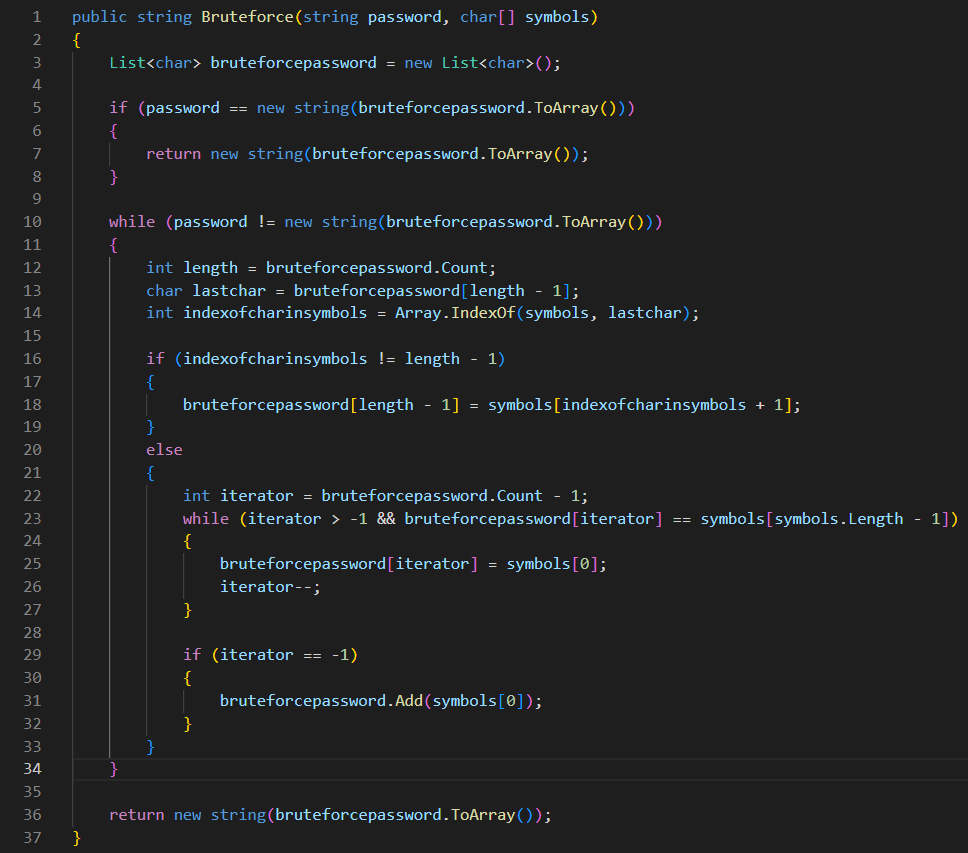
\includegraphics[width=0.7\textwidth]{Bruteforcecode.png}
     \caption[Quellcode des Brute-Force Algorithmus]{selbstgeschriebener Quellcode eines Brute-Force Algorithmus\protect\footnotemark}
     \label{Quellcode des Brute-Force Algorithmus}
  \end{figure}
In der Abbildung ist ein Beispiel Code zusehen, welcher ein Passwort anhand eines Brute-Force Algorithmuses findet. 
Der gegebene Code implementiert eine Funktion namens ``Bruteforce``  in C-Sharp.
Diese Funktion verwendet eine Brute-Force-Methode, um ein Passwort zu erraten, indem sie systematisch alle möglichen Kombinationen von Zeichen ausprobiert.
Der Funktion werden zwei Parameter übergeben: das zu erratende Passwort als Zeichenfolge und ein Array von Symbolen, aus denen die Kombinationen gebildet werden sollen.
Zu Beginn wird eine leere Liste namens ``bruteforcepassword`` erstellt. Dann wird überprüft, ob das gegebene Passwort bereits mit der aktuellen Kombination übereinstimmt. 
Wenn dies der Fall ist, wird die aktuelle Kombination als Zeichenfolge zurückgegeben.
Ansonsten wird eine Schleife gestartet, die solange läuft, bis das gegebene Passwort mit der aktuellen Kombination übereinstimmt. 
In jeder Iteration wird die Länge der aktuellen Kombination bestimmt und das letzte Zeichen abgerufen. 
Es wird der Index dieses Zeichens im Symbol-Array ermittelt.
Wenn der Index nicht gleich der Länge minus eins ist, wird das letzte Zeichen durch das nächste Zeichen im Symbol-Array ersetzt.
Wenn der Index gleich der Länge minus eins ist, bedeutet dies, dass das letzte Zeichen bereits das letzte verfügbare Symbol ist. 
In diesem Fall wird ein Iterator initialisiert, der vom Ende der aktuellen Kombination bis zum Anfang durchläuft. 
Solange das aktuelle Zeichen das letzte verfügbare Symbol ist, wird es durch das erste Symbol im Symbol-Array ersetzt. 
Wenn der Iterator den Anfang erreicht und das aktuelle Zeichen immer noch das letzte Symbol ist, wird das erste Symbol am Ende der aktuellen Kombination hinzugefügt.
Nachdem die Schleife beendet ist und das Passwort gefunden wurde, wird die aktuelle Kombination als Zeichenfolge zurückgegeben.
\subsection{Dictionary Attacks}
\subsubsection{Defintion}
Ein Dictionary-Angriff, auch als Wörterbuch-Angriff bezeichnet, ist eine Methode, um Passwörter oder Schlüssel durch systematisches Ausprobieren einer Liste häufig verwendeter Wörter, Phrasen oder Passwortkombinationen zu knacken.
Bei einem Dictionary-Angriff wird eine vordefinierte Liste, auch als Wörterbuch oder Dictionary bezeichnet, verwendet, die potenzielle Passwörter oder Schlüssel enthält. 
Diese Liste kann verschiedene Formen annehmen, wie beispielsweise eine Sammlung häufig verwendeter Wörter, bekannte Passwörter, gebräuchliche Phrasen oder Kombinationen aus Wörtern und Zahlen.
Der Angriff erfolgt, indem das Programm oder Skript die Liste der Wörter systematisch mit dem Ziel durchprobiert, das Passwort oder den Schlüssel zu finden. 
Es werden verschiedene Variationen und Kombinationen der Wörter aus dem Wörterbuch ausprobiert, einschließlich der Verwendung von Zahlen, Sonderzeichen und Groß- oder Kleinschreibung.
\subsubsection{Funktionsweise}
Die Abbildung veranschaulicht die Funktionsweise eines einfachen Dictionary-Attack-Algorithmus.
\begin{figure}[H]
    \centering
      \includegraphics[width=0.7\textwidth]{dictionary.png}
     \caption[Quellcode eines Dictionary Algorithmus]{selbstgeschriebener Quellcode eines Dictionary Algorithmus\protect\footnotemark}
     \label{Quellcode eines Dictionary Algorithmus}
  \end{figure}
  In diesem Beispielcode wird eine Methode "DictionaryAttack" implementiert, die ein Passwort und eine Liste von Wörtern als Parameter akzeptiert. 
  Der Code durchläuft anschließend jedes Wort in der Liste und vergleicht es mit dem gegebenen Passwort.
  Wenn das Passwort mit einem Wort aus der Liste übereinstimmt, wird das gefundene Wort als Ergebnis zurückgegeben. 
  Andernfalls wird null zurückgegeben, wenn keine Übereinstimmung gefunden wurde.
\subsection{Komplexität von Passwörtern}
Die Anzahl der möglichen Lösungen für ein Passwort kann durch die folgende Formel berechnet werden: Kombinationen = Zeichenanzahl \textsuperscript{Passwortlänge} \footcite[Vgl][S. 2]{ETHZürich}. 
Diese Formel ermöglicht die Untersuchung der verschiedenen Kombinationsmöglichkeiten von Passwörtern. Dabei werden die Ziffern betrachtet, die aus 10 verschiedenen Symbolen bestehen. 
Ebenso werden die Kleinbuchstaben der deutschen Sprache ohne Sonderzeichen berücksichtigt, die aus 26 Symbolen bestehen. 
Zusätzlich werden auch Kleinbuchstaben, Großbuchstaben und Ziffern betrachtet, wodurch sich eine Menge von 62 verschiedenen Symbolen ergibt.
\newpage
\begin{table}[h]
    \centering
    \begin{tabular}{ |c|c|c|c| } 
     \hline
     \textbf{Passwortlänge} & \textbf{Ziffern} & \textbf{Kleinbuchstaben} & \textbf{Kleinbuchstaben, Großbuchstaben und Ziffern}\\ 
     \hline
     1 & $10^1$ & 26 & 62 \\
     2 & $10^2$ & 676 & 3,844 \\
     3 & $10^3$ & 17,576 & 238,328 \\
     4 & $10^4$ & 456,976 & 14,776,336 \\
     5 & $10^5$ & 11,881,376 & 916,132,832 \\
     6 & $10^6$ & 308,915,776 & 56,800,235,584 \\
     7 & $10^7$ & 8,031,810,176 & 3,521,614,606,208 \\
     8 & $10^8$ & 208,827,064,576 & 218,340,105,584,896 \\
     9 & $10^9$ & 5,429,503,678,976 & 13,537,086,546,263,552 \\
     10 & $10^{10}$ & 141,167,095,653,376 & 839,299,365,868,340,224 \\
     11 & $10^{11}$ & 3,670,344,486,987,776 & 52,031,252,847,222,976,512 \\
     12 & $10^{12}$ & 95,428,956,661,682,176 & 3,226,266,762,397,899,821,824 \\
     \hline
    \end{tabular}
    \caption[Kombinationen von Passwörtern]{Kombinationsmöglichkeiten von Passwörtern}
\end{table}
Interessant ist die Passwortlänge von acht, da ein WPA2-Passwort mindestens aus acht Zeichen bestehen muss. 
Bei der Betrachtung der möglichen Kombinationen wird deutlich, dass bei Verwendung von nur Ziffern 10 Millionen Möglichkeiten existieren. 
Im Vergleich dazu gibt es mehr als das 2.000-fache an Möglichkeiten bei Verwendung von Kleinbuchstaben. 
Wenn wir die Kombination von Kleinbuchstaben, Großbuchstaben und Ziffern betrachten, ergibt sich ein Unterschied, der größer als der Faktor 1.000 ist.
\subsection{WPA 2}
WPA2 (Wi-Fi Protected Access 2) ist ein Sicherheitsprotokoll, das in Wi-Fi-Netzwerken verwendet wird, um die Vertraulichkeit und Integrität der drahtlosen Kommunikation zu gewährleisten. 
Es ist der Nachfolger von WPA und bietet eine stärkere Verschlüsselung und verbesserte Sicherheitsfunktionen.
Die Funktionsweise von WPA2 basiert auf einem Vier-Wege-Handshake, der zwischen dem Client (z. B. ein Laptop oder ein Smartphone) und dem Access Point (der drahtlosen Basisstation) stattfindet. 
Der Handshake ermöglicht es beiden Parteien, sich gegenseitig zu authentifizieren und einen gemeinsamen geheimen Sitzungsschlüssel zu etablieren, der für die Verschlüsselung des Datenverkehrs verwendet wird.
WPA2 verwendet zur Verschlüsselung des Passworts den PBKDF2 (Password-Based Key Derivation Function 2)-Algorithmus. Bei PBKDF2 handelt es sich um einen Algorithmus zur Derivation von Schlüsseln basierend auf einem Passwort.

Der Schlüssel für die Verschlüsselung setzt sich dabei aus verschiedenen Komponenten zusammen, nämlich dem Passwort selbst, dem Salt (einem zufälligen Wert), der Anzahl der Iterationen, der verwendeten Hash-Funktion und der Länge des abgeleiteten Schlüssels.
Diese Parameter werden in der Formel key = (password, salt, iterations-count, hash-function, derived-key-len) festgelegt. \footcite{PBKDF2}
\subsection{Rainbow Tables}
\subsubsection{Definition}
Die Rainbow-Tabelle, auch bekannt als Regenbogentabelle, ist eine Datenstruktur, die von Philippe Oechslin entwickelt wurde \cite{Rainbow}. 
Sie ermöglicht eine effiziente und speichersparende Suche nach der ursprünglichen Zeichenfolge, in der Regel ein Passwort, basierend auf einem gegebenen Hashwert. 
Die Rainbow-Tabelle ist eine bedeutende technologische Entwicklung im Bereich der kryptografischen Sicherheit und spielt eine wichtige Rolle bei der Entschlüsselung von Passwörtern und der Sicherheitsanalyse von Hashfunktionen.
\subsubsection{WPA2}
Im Kontext von WPA2 werden Rainbow-Tabellen vor dem Angriff auf das WPA2-Netzwerk neu generiert. 
Beim Erzeugen des Schlüssels wird folgende Formel verwendet: key = pbkdf2(Passwort, SSID, 4096, HMAC-SHA1, 256). 
Die SSID des WLANs wird als Teil des Schlüssels verwendet, um eine eindeutige Verknüpfung zwischen dem Passwort und dem Netzwerk herzustellen. 
Vor dem Angriff können mit Hilfe von Techniken wie der Dictionary-Attack oder Brute-Force viele Schlüssel-Hashwert-Paare erzeugt werden.
Im 4-Wege-Handshake, der zur Authentifizierung zwischen dem Access Point und dem Client stattfindet, wird das verhashte Passwort aufgezeichnet. 
In der dritten Nachricht des 4-Wege-Handshakes, dem EAPOL-Key, ist der PTK (Pairwise Transient Key) enthalten. Der PTK setzt sich aus dem PMK (Pairwise Master Key), zwei zufälligen Zahlen, die zuvor ausgetauscht wurden, sowie den MAC-Adressen des Benutzers und des Access Points zusammen. \footcite[VGL]{professional}
Der PMK ist das verhashte Passwort, das in der Rainbow-Tabelle gesucht werden kann. 
Wenn ein passender Hashwert in der Rainbow-Tabelle gefunden wird, bedeutet dies, dass das ursprüngliche Passwort ebenfalls gefunden wurde. 
Die Rainbow-Tabelle ermöglicht es Angreifern, auf effiziente Weise Passwörter zu entschlüsseln und somit Zugang zu einem geschützten WPA2-Netzwerk zu erlangen. 


    
    
 

\newpage
\section{Ist- und Problemanalyse}


 

\newpage
\section{Lösungskonzept}

 

\newpage
\section{Fazit}

 

% -----------------------------------------------------

\label{pagesForDeclaration}

\clearpage
\pagenumbering{Roman}
\setcounter{page}{\value{pageNumber}}

\section*{\referenceHeading}
\addcontentsline{toc}{section}{\referenceHeading}
\defbibheading{books}{\noindent\large\textbf{Bücher}}
\printbibliography[type=book, heading=books]

\defbibheading{incollection}{\noindent\large\textbf{Sammelwerke}}
\printbibliography[type=incollection, heading=incollection]

\defbibheading{article}{\noindent\large\textbf{Artikel}}
\printbibliography[type=article, heading=article]

\defbibheading{online}{\noindent\large\textbf{Internetquellen}}
\printbibliography[type=online, heading=online]

\defbibheading{interview}{\noindent\large\textbf{Interviews}}
\printbibliography[type=interview, heading=interview]

\defbibheading{internal}{\noindent\large\textbf{Interne Quellen}}
\printbibliography[type=unpublished, heading=internal]

\newpage

\section*{\appendixHeading}
\addcontentsline{toc}{section}{\appendixHeading}

\begin{enumerate}
\item Digitale Version der Arbeit
\item Interviews
\begin{enumerate}
\item Expertmann 2018
\end{enumerate}
\end{enumerate}

 
\end{document}